\subsection{Corwin Perren}
\subsubsection{Week 1}
The first week Chris, Ken, and I met in Graf 306 after the first capstone class of the term. During this meeting I showed them the Rover hardware, ground station hardware, and the general workspace that we'd be spending much time in for the next two terms. We then also came up with a work schedule consisting of roughly five hours or more a day on Tuesdays, Thursdays, and Saturdays. Initial tasks we're divvied up and we began work on our respective parts. My task was to continue work on the video display systems that I'd written testing code for the previous term. The primary item I got working this week was adding camera name labels to the stream so that it would be easy to tell what camera was being viewed, even if the user changed where the stream was displayed. I also added FPS counters to my development streams so I could ensure they were displaying at 30 FPS or above, and made some code adjustments for efficiency. Plans were made to begin development of the auto quality adjustment systems for subsequent weeks. During this week, only a single video stream was being displayed.

\subsubsection{Week 2}
During week 2, I continued work on the video receiving and display class, starting by testing its reliability with network disconnections and running the software for an extended period of time. Once semi-verified, I began work refactoring my prototype class into two new classes, a VideoReceiver class and VideoCoordinator class. The VideoReceiver class will handle the low level grabbing of video frames from the ROS topic, adjusting which resolution it's subscribed to, and automatic quality adjustments based on changes to frame rates. It will also allow each instance's stream to be disabled, so that network bandwidth is not being used when the stream is not being displayed. 
\\
The VideoCoordinator class determines which video streams are available upon launch, and creates instantiations of the VideoReceiver classes as necessary. It also handles displaying the frames provided by the VideoReceiver classes in the QLabels on the GUI that are being used to view the streams. Users can also left-click on the stream windows to tell the VideoCoordinator to change what stream is being displayed. A right-click will allow a particular stream to be disabled to save on network bandwidth. 
\\
This week I also began refactoring the core program code structure and launch file so that we would have a solid foundation to work off of, and to allow us to more easily integrate our classes as the terms progress.

\subsubsection{Week 3}
I finished work on the core program structure during the beginning of this week, and added an additional feature to ensure the Rover itself was present on the network before starting, as the GUI is useless without it. It will also make it easy to tell if the radios are functioning down the line. As part of this rework, I added a shared object to be passed around to the  classes we make so they have access to GUI elements, other instances of classes, and each other. This is mainly needed to make the signal/slot connections that Qt is based around.
\\
I made significant progress on writing the VideoReceiver and VideoCoordinator classes this week. Namely, the VideoCoordinator class could successfully dynamically adjust to the number of video streams present on launch, as opposed to hard coding the cameras in. To go along with this, changing which stream was displayed became possible on all three video displays, as well as disabling streams with the right-click described before. When disabled, the video now completely kills that streams connection to the Rover, so its bandwidth usage drops to zero. In a similar vein, if the user is cycling video streams and a particular stream has not been explicitly disabled, but is not active on a video display, the stream is "sleeped" by disabling the stream. Once it is being viewed again, the stream automatically re-activates.
\\
To finish off the week, I made placeholder blocks in the GUI design files that matched our design document layout. This was so that it would be easier to drop in actually useful GUI elements as they are designed.
\begin{figure}[h!]
  \centering
  \captionsetup{justification=centering}
  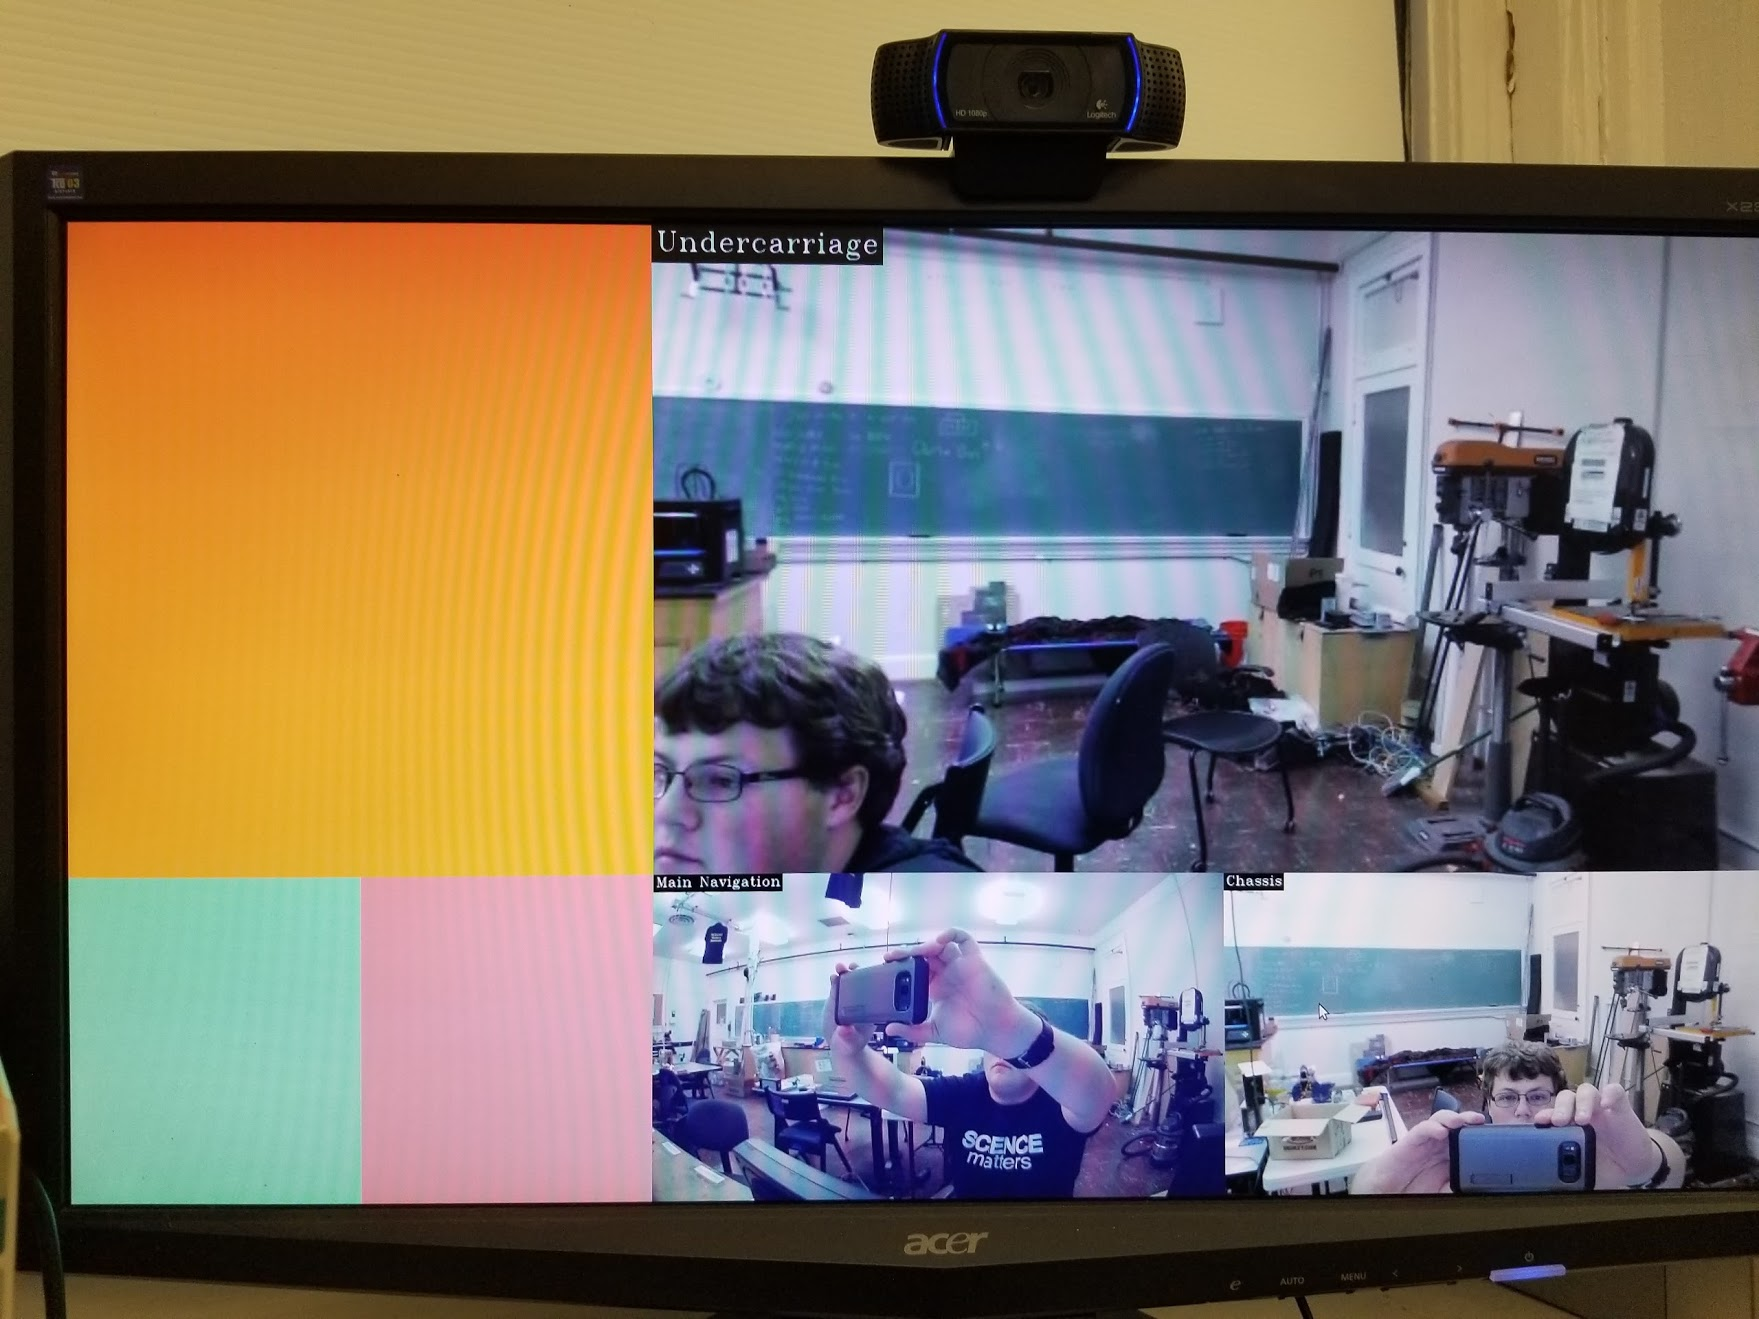
\includegraphics[width=0.5\textwidth]{figures/video_working}
  \caption{Three streams working}
\end{figure}

\subsubsection{Week 4}
This week, I began a slight departure from pure ground station work as it was becoming apparent that progress on the main Rover software and electrical systems were behind. Talking with the team lead, Nick McComb, it was determined that my time for a week or two would be best spent helping write ROS nodes for the Rover or firmware for micro-controllers. With this in mind, I worked on getting the GPS and Inertial Measurement Unit attached to a Teensy 3.2 sending data to the Rover. This involved making modifications to a Modbus RTU library so that it would be compatible with the Teensys. Once the firmware was working and properly sending out data, I then wrote a receiving node for ROS to take in the GPS and IMU data over serial and broadcast it to the rest of the ROS systems. This step was particularly helpful as our team now has working GPS data to use for mapping and waypoint systems on the ground station.I also began minimal work on a mock motor driver node for the Rover, so that we could more quickly be able to test remote driving.

\subsubsection{Week 5}
Week 5 was a particularly slow week as I had midterms. Very similarly to the previous week, I decided that my time was best spent trying to help with other aspects of the team, in this case electrical. The Rover's main control board, Iris, needed to be assembled and I have extensive soldering experience so I spent 17 hours over two days assembling, testing, and fixing problems with this main control board. As everything on the Rover has to communicate through this board, it is essential to have it working both for the main software team and capstone. I wrote a simple motor driving ROS node that communicated with another Teensy microcontroller attached to a motor driver and test motor.
\begin{figure}[h!]
  \centering
  \captionsetup{justification=centering}
  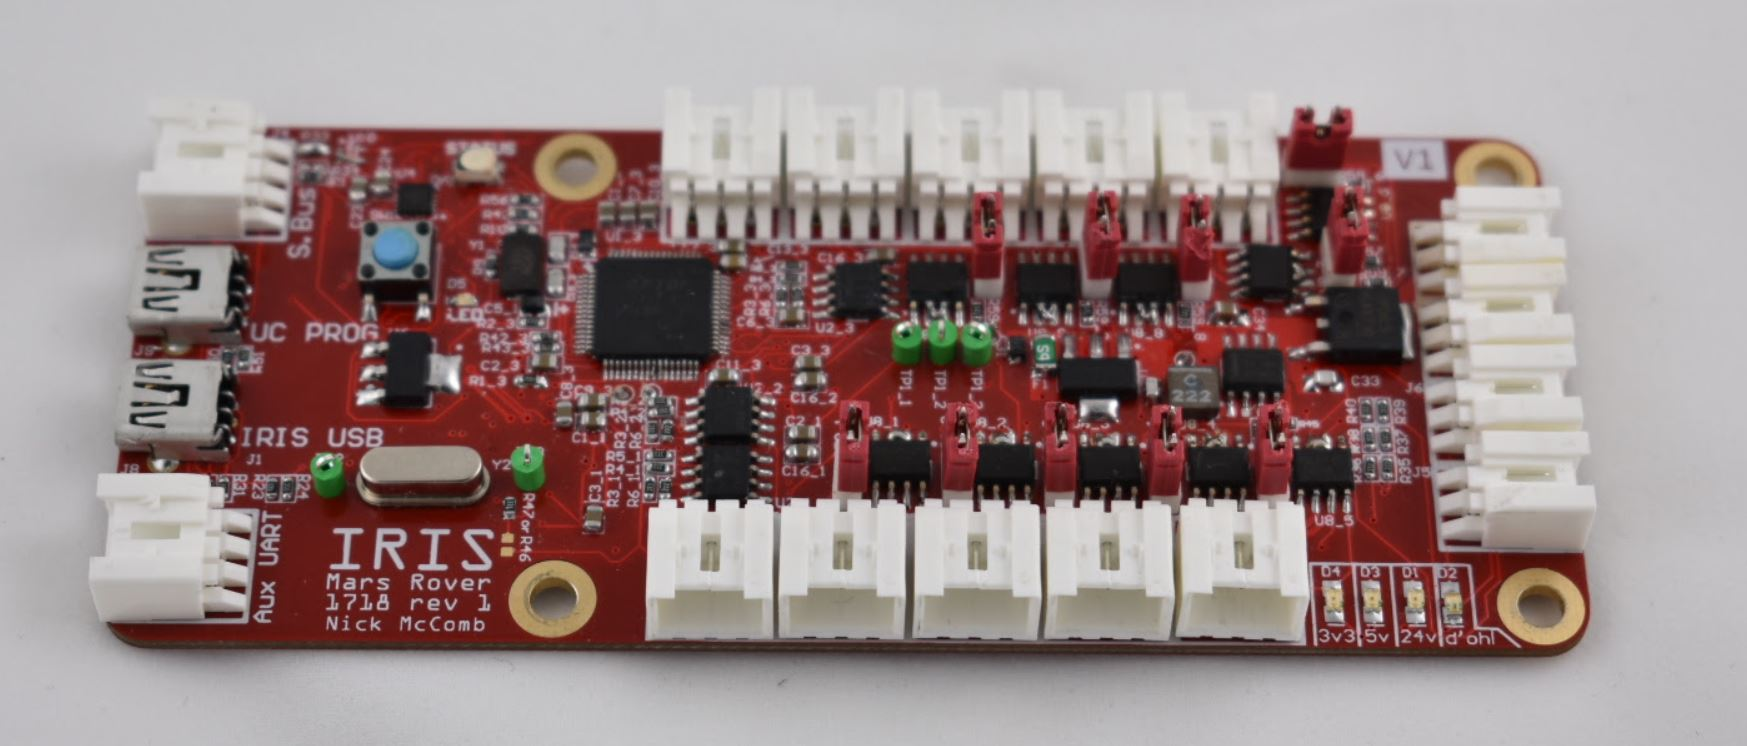
\includegraphics[width=0.5\textwidth]{figures/iris}
  \caption{Iris after assembly}
\end{figure}

\subsubsection{Week 6}
The final week, ending in this report, was mostly spent working on the rough draft of the Expo poster. Our team filled out the poster with all the major information and graphics and should only require minimal modification for the final revision. Due to having gotten a simple motor driver node working the previous week, I did write a simple example python script to read in joystick data on the ground station and broadcast it to the Rover, properly moving the motor. This was a very simple demo however, and needs a finalized version of the ROS motor driving nodes on the Rover in order to be integrated into the actual ground station software.

\subsubsection{Github Commits}
\begin{center}
\begin{tabular}{l l l l}	\textbf{Detail} & \textbf{Author} & \textbf{Date} &\textbf{Description}\\\hline
\href{https://github.com/OSURoboticsClub/Rover_2017_2018/commit/0f8103eb2dc990541e7f181bd4ac8afa3c5b06a1}{0f8103e} & Corwin Perren & 2018-01-12 00:43 &Changed the launch file to have the correct camera names.\\\hline
\href{https://github.com/OSURoboticsClub/Rover_2017_2018/commit/b2c495e6b69c4f38cd2d4e6e1ac0a48703fac9f1}{b2c495e} & Corwin Perren & 2018-01-11 16:45 &Added names to the testing images and fps counters\\\hline
\href{https://github.com/OSURoboticsClub/Rover_2017_2018/commit/53d8de2ea80d6034f0906da0aa5e2d3df0dd6aae}{53d8de2} & Corwin Perren & 2018-01-13 21:50 &Changed one of the camera names\\\hline
\href{https://github.com/OSURoboticsClub/Rover_2017_2018/commit/2e40a51e830b5ffffd97820d597b73360b716d12}{2e40a51} & Corwin Perren & 2018-01-14 03:01 &Updated UDEV rules for camera names\\\hline
\href{https://github.com/OSURoboticsClub/Rover_2017_2018/commit/c49b90b038ad2b31b2b1643f9f55f86c5cdfa658}{c49b90b} & Corwin Perren & 2018-01-20 17:16 &Added thrid resolution for cameras\\\hline
\href{https://github.com/OSURoboticsClub/Rover_2017_2018/commit/08fc436fa277f839826840774823bae37c9bc45e}{08fc436} & Corwin Perren & 2018-01-22 22:42 &Updated UI Files\\\hline
\href{https://github.com/OSURoboticsClub/Rover_2017_2018/commit/4d071d304ed3781c89f4a5067644981131a33226}{4d071d3} & Corwin Perren & 2018-01-23 09:07 &Updated layout of the main launcher, as well as ui files.\\\hline
\href{https://github.com/OSURoboticsClub/Rover_2017_2018/commit/60ea2d9339e11a6ec749b47d5b5487ccb39d8f09}{60ea2d9} & Corwin Perren & 2018-01-23 09:27 &Added a dark stylesheet so things look nice\\\hline
\href{https://github.com/OSURoboticsClub/Rover_2017_2018/commit/6270f7380f6fd9b73c99193c93860d4042816e7b}{6270f73} & Corwin Perren & 2018-01-23 10:22 &Launching RoverVideeoCoordinator. Added working logging... \\\hline
\href{https://github.com/OSURoboticsClub/Rover_2017_2018/commit/03706408d374a025982071ab5414694a2742d8ca}{0370640} & Corwin Perren & 2018-01-23 12:54 &Added check for ros master on startup. More work on video...\\\hline
\href{https://github.com/OSURoboticsClub/Rover_2017_2018/commit/05c65645e9c4a87a6571797f7dd8680858f095f2}{05c6564} & Corwin Perren & 2018-01-23 14:44 &RoverVideoCoordinator now kind of working with VideoReceiver...\\\hline
\href{https://github.com/OSURoboticsClub/Rover_2017_2018/commit/b85319665e7fa439f4834266e504547d630671eb}{b853196} & Corwin Perren & 2018-01-23 17:08 &Got changing video sources working, along with showing the...\\\hline
\href{https://github.com/OSURoboticsClub/Rover_2017_2018/commit/6297a2af444c42c48861fc4852042402748274e5}{6297a2a} & Corwin Perren & 2018-01-25 15:46 &Video modifications and last changes\\\hline
\href{https://github.com/OSURoboticsClub/Rover_2017_2018/commit/fc1b41178cea41bbf1d846e0178cee1cd1d800f9}{fc1b411} & Corwin Perren & 2018-01-25 15:49 &Changed layout for organizational coherence.\\\hline
\href{https://github.com/OSURoboticsClub/Rover_2017_2018/commit/006f11af653ba82b0984a2de92f99dc3f240cdd0}{006f11a} & Corwin Perren & 2018-01-25 16:11 &Auto-sleep of background cameras works. Dynamic changing of...\\\hline
\href{https://github.com/OSURoboticsClub/Rover_2017_2018/commit/0e72b84a930ab4a58539d535a9a177c3a0cb9f8b}{0e72b84} & Corwin Perren & 2018-01-25 16:17 &Removed workspace files\\\hline
\href{https://github.com/OSURoboticsClub/Rover_2017_2018/commit/71aca163d60f6ea6bacbde141f42a9d693305c5d}{71aca16} & Corwin Perren & 2018-01-25 16:20 &Fixing things.\\\hline
\href{https://github.com/OSURoboticsClub/Rover_2017_2018/commit/219bc0956cbec27066b3f25de0edcc7397a7ef12}{219bc09} & Corwin Perren & 2018-01-25 17:55 &Everything ready to do sensing of frame rates to adjust quality...\\\hline
\href{https://github.com/OSURoboticsClub/Rover_2017_2018/commit/bb8bae2f55caca5f45d0ed77e9ab8ad933ccb8fc}{bb8bae2} & Corwin Perren & 2018-02-03 15:09 &Removed ublox. Added rover\_drive\\\hline
\href{https://github.com/OSURoboticsClub/Rover_2017_2018/commit/940d2782c361acee060488d8b07636eb3fc2eb7f}{940d278} & Corwin Perren & 2018-02-03 17:12 &Added beginnings of getting motor control working from within...\\\hline
\href{https://github.com/OSURoboticsClub/Rover_2017_2018/commit/ad4bf7d74c408d05a6d1788f1b981c0c8380865d}{ad4bf7d} & Corwin Perren & 2018-02-11 21:18 &Some new drive code. Firmware too, but that's not up yet.\\\hline
\href{https://github.com/OSURoboticsClub/Rover_2017_2018/commit/c90247643f816b5add089c604804ead6e8a73b3e}{c902476} & Corwin Perren & 2018-02-12 21:03 &workspace\\\hline
\href{https://github.com/OSURoboticsClub/Rover_2017_2018/commit/b5be2a6f2472909ed06ee3535c4eec78f6c601ab}{b5be2a6} & Corwin Perren & 2018-02-12 21:04 &Merge branch 'video\_testing'\\\hline
\href{https://github.com/OSURoboticsClub/Rover_2017_2018/commit/aca4c0627c3ce4ed2f6b3c4513e8ffccbb2b2277}{aca4c06} & Corwin Perren & 2018-02-13 13:20 &Map now loads. Changed launcher to match monitors.\\\hline
\href{https://github.com/OSURoboticsClub/Rover_2017_2018/commit/d13a0d2d69b27b816e33b2eade6f1e9f102bc0ef}{d13a0d2} & Corwin Perren & 2018-02-14 18:35 &Updated UI Files. Getting closer to actual layout.\\\hline
\href{https://github.com/OSURoboticsClub/Rover_2017_2018/commit/f009383b3eb6f0868cc842b70d3430cd41be3816}{f009383} & Corwin Perren & 2018-02-14 18:39 &Added missing compass image\\\hline
\href{https://github.com/OSURoboticsClub/Rover_2017_2018/commit/4698723bb0e747fb52d420056f2822ff04005f9d}{4698723} & Corwin Perren & 2018-02-14 18:51 &Changed right screen so it color matches\\\hline
\href{https://github.com/OSURoboticsClub/Rover_2017_2018/commit/9b3fd50188b3a7504998bac4456ce3717f8a827b}{9b3fd50} & Corwin Perren & 2018-02-14 19:52 &Very rough joystick driving working\\\hline
\href{https://github.com/OSURoboticsClub/Rover_2017_2018/commit/b54c8c38566fa1de3f41249c2f4ac9f58b08f4ab}{b54c8c3} & Corwin Perren & 2018-02-15 18:33 &Updated README for ground station.\\\hline
\end{tabular}
\end{center}